% Options for packages loaded elsewhere
\PassOptionsToPackage{unicode}{hyperref}
\PassOptionsToPackage{hyphens}{url}
\documentclass[12pt, ]{article}

\usepackage{mathtools}
\usepackage{amsmath}
\usepackage{amsthm}
\usepackage{amssymb}
\usepackage[italicdiff]{physics}
\mathtoolsset{showonlyrefs}

% SPACING AND FONTS %%%%%%%%%%%%%%%%%%%%%%%%%%%%%%%%%%%%%%%%%%%%%%%%%%%%%%%%%%%%
\usepackage{iftex}
% CAREFUL: the order of font includes here is very important!
\ifPDFTeX
  \usepackage[OT1,T1]{fontenc}
  \usepackage[utf8]{inputenc}
  \usepackage{textcomp} % provide euro and other symbols
    \usepackage[p,osf,swashQ]{cochineal}
  \usepackage[cochineal,vvarbb]{newtxmath}
      \usepackage[scale=0.95]{biolinum}
    \usepackage[scale=0.95,varl]{inconsolata}
\else % if luatex or xetex
  \usepackage[scale=0.95,varl]{inconsolata}
  \usepackage{newpxtext}
  \usepackage{mathpazo}
    \usepackage[scale=0.95]{biolinum}
  \fi
\ifLuaTeX
  \usepackage{selnolig}  % disable illegal ligatures
\fi
\IfFileExists{microtype.sty}{% use microtype if available
  \usepackage[]{microtype}
  \UseMicrotypeSet[protrusion]{basicmath} % disable protrusion for tt fonts
}{}

\setlength{\parindent}{0pt}
\setlength{\parskip}{10pt plus 2pt minus 2pt}
\setlength{\emergencystretch}{3em} % prevent overfull lines
\widowpenalty=10000
\clubpenalty=10000
\flushbottom
\allowdisplaybreaks
\sloppy


% CORE PACKAGES %%%%%%%%%%%%%%%%%%%%%%%%%%%%%%%%%%%%%%%%%%%%%%%%%%%%%%%%%%%%
\usepackage[dvipsnames,svgnames,x11names]{xcolor}
\usepackage[lmargin=1.5in,rmargin=1.5in,tmargin=1.2in,bmargin=1.2in]{geometry}
\usepackage[format=plain,
  labelfont={bf,sf,small,singlespacing},
  textfont={sf,small,singlespacing},
  justification=justified,
  margin=0.25in]{caption}

% SECTIONS AND HEADINGS %%%%%%%%%%%%%%%%%%%%%%%%%%%%%%%%%%%%%%%%%%%%%%%%%%%%%%%%
\setcounter{secnumdepth}{4}
\usepackage{sectsty}
\usepackage[compact]{titlesec}
% short title
\makeatletter
\newcommand\@shorttitle{}
\newcommand\shorttitle[1]{\renewcommand\@shorttitle{#1}}
\usepackage{fancyhdr}
\fancyhf{}
\pagestyle{fancy}
\renewcommand{\headrulewidth}{0pt}
\fancyheadoffset{0pt}
%\lhead{\scshape \@shorttitle}
%\rhead{\scshape\today}
\cfoot{\thepage}
\makeatother
% abstract styling
\renewenvironment{abstract}{
  \centerline
  {\large\sffamily\bfseries Abstract}\vspace{-1em}
  \begin{quote}\small
}{
  \end{quote}
}

% PANDOC INCLUDES %%%%%%%%%%%%%%%%%%%%%%%%%%%%%%%%%%%%%%%%%%%%%%%%%%%%%%%%%%%%%%

\providecommand{\tightlist}{%
  \setlength{\itemsep}{0pt}\setlength{\parskip}{0pt}}\usepackage{longtable,booktabs,array}
\usepackage{calc} % for calculating minipage widths
% Correct order of tables after \paragraph or \subparagraph
\usepackage{etoolbox}
\makeatletter
\patchcmd\longtable{\par}{\if@noskipsec\mbox{}\fi\par}{}{}
\makeatother
% Allow footnotes in longtable head/foot
\IfFileExists{footnotehyper.sty}{\usepackage{footnotehyper}}{\usepackage{footnote}}
\makesavenoteenv{longtable}
\usepackage{graphicx}
\makeatletter
\def\maxwidth{\ifdim\Gin@nat@width>\linewidth\linewidth\else\Gin@nat@width\fi}
\def\maxheight{\ifdim\Gin@nat@height>\textheight\textheight\else\Gin@nat@height\fi}
\makeatother
% Scale images if necessary, so that they will not overflow the page
% margins by default, and it is still possible to overwrite the defaults
% using explicit options in \includegraphics[width, height, ...]{}
\setkeys{Gin}{width=\maxwidth,height=\maxheight,keepaspectratio}
% Set default figure placement to htbp
\makeatletter
\def\fps@figure{htbp}
\makeatother
% END PANDOC %%%%%%%%%%%%%%%%%%%%%%%%%%%%%%%%%%%%%%%%%%%%%%%%%%%%%%%%%%%%%%%%%%%

% USER INCLUDES %%%%%%%%%%%%%%%%%%%%%%%%%%%%%%%%%%%%%%%%%%%%%%%%%%%%%%%%%%%%%%%%
% additional LaTeX code for the "preamble" goes here
\usepackage{float} \floatplacement{table}{H}
\makeatletter
\makeatother
\makeatletter
\makeatother
\makeatletter
\@ifpackageloaded{caption}{}{\usepackage{caption}}
\AtBeginDocument{%
\ifdefined\contentsname
  \renewcommand*\contentsname{Table of contents}
\else
  \newcommand\contentsname{Table of contents}
\fi
\ifdefined\listfigurename
  \renewcommand*\listfigurename{List of Figures}
\else
  \newcommand\listfigurename{List of Figures}
\fi
\ifdefined\listtablename
  \renewcommand*\listtablename{List of Tables}
\else
  \newcommand\listtablename{List of Tables}
\fi
\ifdefined\figurename
  \renewcommand*\figurename{Figure}
\else
  \newcommand\figurename{Figure}
\fi
\ifdefined\tablename
  \renewcommand*\tablename{Table}
\else
  \newcommand\tablename{Table}
\fi
}
\@ifpackageloaded{float}{}{\usepackage{float}}
\floatstyle{ruled}
\@ifundefined{c@chapter}{\newfloat{codelisting}{h}{lop}}{\newfloat{codelisting}{h}{lop}[chapter]}
\floatname{codelisting}{Listing}
\newcommand*\listoflistings{\listof{codelisting}{List of Listings}}
\makeatother
\makeatletter
\@ifpackageloaded{caption}{}{\usepackage{caption}}
\@ifpackageloaded{subcaption}{}{\usepackage{subcaption}}
\makeatother
\makeatletter
\@ifpackageloaded{tcolorbox}{}{\usepackage[skins,breakable]{tcolorbox}}
\makeatother
\makeatletter
\@ifundefined{shadecolor}{\definecolor{shadecolor}{rgb}{.97, .97, .97}}
\makeatother
\makeatletter
\makeatother
\makeatletter
\makeatother
% END USER INCLUDES %%%%%%%%%%%%%%%%%%%%%%%%%%%%%%%%%%%%%%%%%%%%%%%%%%%%%%%%%%%%

% BIBLIOGRAPHY %%%%%%%%%%%%%%%%%%%%%%%%%%%%%%%%%%%%%%%%%%%%%%%%%%%%%%%%%%%%%%%%%
\usepackage[]{natbib}
\bibliographystyle{apalike}

% Give it this name so that it works with ::: #refs
\newenvironment{CSLReferences}[2]{
\bibliography{bibliography.bib}
\clearpage
}{}

% LINKS %%%%%%%%%%%%%%%%%%%%%%%%%%%%%%%%%%%%%%%%%%%%%%%%%%%%%%%%%%%%%%%%%%%%%%%%
\usepackage{hyperref}
\usepackage{url}
\hypersetup{
  pdftitle={Political Exchange Dynamics: Unveiling Heterogeneous Effects on City Mayor Promotion Prospects in China},
  pdfauthor={Ezeriki Emetonjor},
  colorlinks=true,
  linkcolor={blue},
  filecolor={Maroon},
  citecolor={VioletRed4},
  urlcolor={DodgerBlue4},
  pdfcreator={LaTeX via pandoc}}

% TITLE, AUTHOR, DATE %%%%%%%%%%%%%%%%%%%%%%%%%%%%%%%%%%%%%%%%%%%%%%%%%%%%%%%%%%
\title{\sffamily\bfseries\huge\parfillskip=0pt
\rightskip=0pt plus .5\textwidth
\leftskip=0pt plus .5\textwidth
\emergencystretch=.3\textwidth Political Exchange Dynamics: Unveiling
Heterogeneous Effects on City Mayor Promotion Prospects in China}
\shorttitle{Political Exchange Dynamics: Unveiling Heterogeneous Effects on City Mayor Promotion Prospects in China}
\author{\textbf{Ezeriki Emetonjor}
 }
\date{}


\begin{document}
\allsectionsfont{\sffamily}

\maketitle

\begin{abstract}
This research investigates heterogeneous effects within a political
exchange paradigm operative in Chinese local political frameworks
involving Provincial Party Secretaries (PPS) and City Mayors. Expanding
on previous investigations that showed how this political exchange
affects higher infrastructure spending in China relative to other
countries, this study specifically centers on subway infrastructure as a
conduit facilitating the alignment of objectives between PPS and city
mayors, thereby augmenting their prospects for future career
advancements. My findings reveal statistically significant differences
in the efficacy of securing subway project approvals in relation to
tenure, which can greatly influence the promotion likelihood of city
mayors in China. Furthermore, my study confirms that there are no
statistically significant differences based on age.
\end{abstract}

\ifdefined\Shaded\renewenvironment{Shaded}{\begin{tcolorbox}[borderline west={3pt}{0pt}{shadecolor}, enhanced, boxrule=0pt, interior hidden, sharp corners, frame hidden, breakable]}{\end{tcolorbox}}\fi



% USER BODY %%%%%%%%%%%%%%%%%%%%%%%%%%%%%%%%%%%%%%%%%%%%%%%%%%%%%%%%%%%%%%%%%%%%

\newpage{}

\hypertarget{introduction}{%
\section{Introduction}\label{introduction}}

Within the scope of this investigation, I identify divergent effects
inherent in a political exchange model, catalyzing economic development
in the localities served by participating politicians. This intricate
interplay not only fosters public good provision but also yields private
advantages in terms of enhanced promotion prospects for the involved
parties. The government's pivotal role in furnishing public goods,
particularly substantial ones with broad societal impact, is
well-acknowledged. Yet, at the local level, such as in cities, the
investment trajectory in large-scale public goods, like infrastructure
projects, is often misaligned with the typical tenure of local political
leaders.

Addressing this incompatibility, \citet{lei2022private} conducted an
exploration of China's city politics, where this disjunction appears
notably absent. Their study delves into the nuanced political
transactions between Provincial Party Secretaries (PPS) and City Mayors,
demonstrating a clear association with significantly higher public
infrastructure investments in China as compared to other countries.
\citep{lei2022private}. Their study focuses specifically on subway
infrastructure, given its integral role in fostering economic growth,
the direct participation of city mayors, and the constrained contracting
dynamics that span across cities and time, contingent upon the mayors'
capabilities. One relevant question that emerges from this study
concerns the varying benefits and drawbacks that different kinds of
politicians encounter when they participate in these kinds of political
interactions. Two categories that require careful examination and that
demonstrate related dynamics are age and tenure.

Initially, with a focus on tenure as a pivotal element in this political
exchange paradigm, \citet{guo2009china} investigates the behavior of
county-level political leaders in China. The study reveals a tendency
for increased spending on economically beneficial projects during
crucial junctures in their careers, particularly in the tenure year with
elevated prospects of promotion, notably in the third and fourth years
of their term. In the context of authoritative governance, as observed
in China, politicians' immediate superiors hold the majority of
political influence when it comes to appointing new leaders
\citep{lei2022private, guo2009china}. Consequently, the generation of
positive economic outcomes through large-scale public initiatives
functions as a potent signal of the competence and deserving promotion
of local politicians to their superiors; this highlights the
effectiveness of these signals in comparison to potentially biased
markers such as personality traits or prior experiences, which might not
be able to accurately predict future abilities \citep{guo2009china}.

Given the framework established by the \citet{lei2022private} study, I
anticipate a substantial influence of a city mayor's tenure on subway
infrastructure investment, subsequently impacting their prospects for
future promotion. Consequently, this investigation delves into the
interplay between a mayor's tenure and the successful approval of a
subway infrastructure project. Notably, my findings highlight that city
mayors with tenure spanning up to three or four years, coupled with the
attainment of subway project approvals, experience the highest
likelihood of promotion. This alignment with a political cycle framework
underscores the strategic nature of engaging in local-level investments
during periods offering the greatest prospects for promotion, as
specified in prior research \citep{guo2009china}.

An additional pertinent factor to consider is age, which holds
significant relevance in the broader context of political
representation. The global trend of citizens favoring candidates who
share similar characteristics is a critical aspect, as highlighted by
\citet{sevi2021young}. This preference is grounded in the belief that
candidates with similarities are more inclined to act in the best
interests of the citizens and champion policies beneficial to their
specific demographic. Various dimensions contribute to measures of
representation, including ethnicity, race, and age, as elucidated by
\citet{sevi2021young}. Building upon this, the work of
\citet{lei2022private} provides a valuable case study to empirically
test the hypothesis that voters, or in the context of the Chinese
authoritarian system, those influencing the promotion of political
leaders, are more inclined to select individuals with whom they share
similarities.

Consequently, age proves to be a compelling demographic variable for
examination within the framework of the \citet{lei2022private} study,
given its dynamic nature that evolves over time. This sets it apart from
other human traits such as gender or ethnicity \citep{stockemer2018age}.
According to \citet{stockemer2018age}, middle-aged and wealthy people
often make up the global political elite. This presents a noteworthy
challenge because, just as age evolves, so do ideologies, beliefs, and
perspectives on life. Consequently, young adults often find themselves
at odds with older generations regarding policy and political solutions,
experiencing inadequate representation by their governments in the
current state of affairs \citep{stockemer2018age}. The
\citet{lei2022private} study offers an avenue to explore whether age
groups falling outside the conventional realm of ``politician age'' are
disadvantaged in this political market system.

Building upon the context established in the preceding paragraphs, an
interplay between tenure and age becomes apparent. Younger politicians
are predisposed to having fewer tenure years, and for those just
commencing their careers, they might find themselves a few years ahead
of the conventional promotion schedule. Consequently, securing
infrastructure projects may not wield decisive influence over their
promotion prospects. Moreover, additional hurdles may hinder their
advancement, such as the perceived inexperience commonly associated with
their age. In contrast, senior politicians encounter a diametric
challenge, facing an imminent deadline to demonstrate tangible results
during their remaining time in office. However, the extensive tenure of
older leaders, coupled with their perceived experience and age-related
affinity with political superiors, may render it less challenging for
them to secure opportunities, such as infrastructure contracts, thereby
enhancing their prospects of promotion. Nevertheless, as underscored by
\citet{guo2009china}, there exists a potential downside to investing in
significant public projects during extended tenures, as it may coincide
with missing optimal promotion periods. Additionally, age discrimination
may manifest, with the negative impact of being deemed too old working
against their promotion prospects. Consequently, it is plausible to
anticipate that middle-aged city mayors, strategically aligning with the
peak promotion tenured years, would generally exhibit the highest
likelihood of promotion, attributed to their successful endeavors in
obtaining approval for subway projects. The paper further details the
analysis of data from \citet{lei2022private}, using the
difference-in-differences design to estimate the causal impact of subway
approval on a city mayor's promotion prospects. It also extends the
design to uncover heterogeneous differences within crucial indicators
like tenure and age.

\hypertarget{data-analysis}{%
\section{Data \& Analysis}\label{data-analysis}}

The examination draws upon data obtained from the \citet{lei2022private}
study, utilizing sources such as the China City Statistical Yearbook,
China Urban Construction Yearbook, Chinese Political Elite Database,
among others. These sources collectively compile information on
city-level infrastructure projects, demographic characteristics, and the
past educational and professional experiences of city mayors and PPS
officials \citep{lei2022private}. Table~\ref{tbl-statsumm} provides a
snapshot of some important mayor and city characteristics.

\hypertarget{tbl-statsumm}{}
\begin{longtable}[]{@{}l@{}}
\caption{\label{tbl-statsumm}Summary Statistics}\tabularnewline
\toprule\noalign{}
\endfirsthead
\endhead
\bottomrule\noalign{}
\endlastfoot
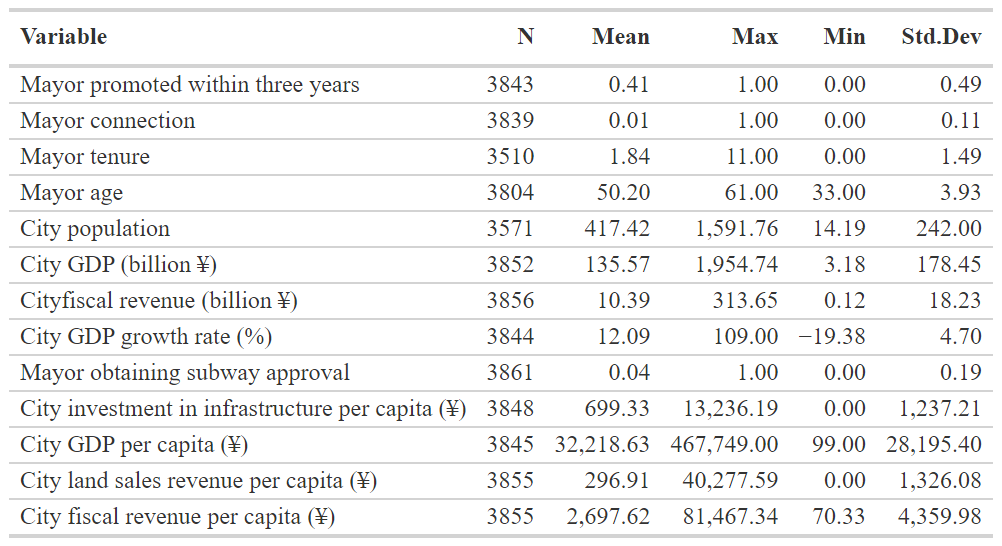
\includegraphics{tables/final_summ_stat.png} \\
\end{longtable}

I replicate the difference-in-differences design from
\citet{lei2022private} and extend it with a focus on heterogeneous
effects related to tenure and age. To capture the nuanced interaction
between tenure, subway approvals, and future promotion, I introduce an
interaction term with the independent variable of interest---Mayor's
subway approval for that city in that year---allowing for an examination
of how the impact of subway approvals varies across different tenures.

\begin{figure}[tbp]

{\centering 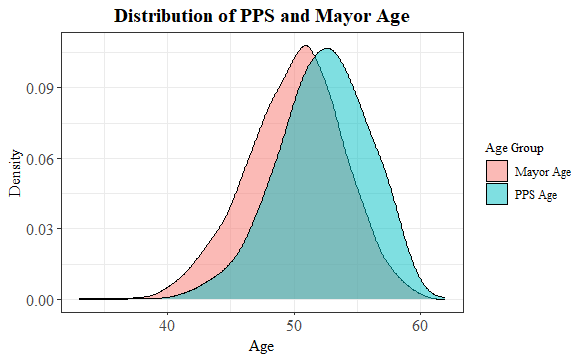
\includegraphics[width=0.6\textwidth,height=\textheight]{figures/age_distribution2.png}

}

\caption{\label{fig-agedist}Age distribution of Provincial Party
Secretaries and City Mayors}

\end{figure}

Concerning age and its interplay with tenure, the distribution of age
for both PPS and city mayors is visualized by Figure~\ref{fig-agedist}.
Notably, the age distribution overlap occurs predominantly within the
range of 45 to 59 years, with a concentration between 48 and 56 years.
Consequently, it is anticipated that city mayors falling within this age
group, closer in age to PPS counterparts, would exhibit higher chances
of promotions, aligning with the earlier hypothesis. Specifically, this
connection may be linked to a significant portion of individuals within
this age bracket concurrently being in their 3rd or 4th years in office,
a period associated with elevated promotion probabilities. To ascertain
the specific effect of the interaction between age and subway approvals
on future promotions, controlling for tenure becomes crucial in order to
isolate that particular effect. To align the data with my hypothesis, I
leverage the existing Age variable in \citet{lei2022private}'s dataset
to construct a distinct grouping variable. This new variable categorizes
ages into six groups, each spanning a five-year range, from the minimum
age of 33 to the maximum age of 62. To ensure non-overlapping bins, the
initial term within each age group is included in the previous bin. The
resulting Age group variable is subsequently incorporated into the
original difference-in-differences design using interaction terms with
the subway approval variable.

\hypertarget{baseline-difference-in-difference-design}{%
\section{Baseline Difference in Difference
Design}\label{baseline-difference-in-difference-design}}

The difference-in-differences design proposed by \citet{lei2022private}
can be expressed through an ordinary least squares regression:
\[P_{ct} = \alpha + \beta_{1}Approval + \gamma X_{c,t - 1} + \eta_{c} + \theta_{t} + \epsilon_{ct},\]
where \(P_{ct}\) denotes the future promotion of the city mayor in 3
years for city c in year t. The City fixed effects (\(\eta_{c}\))
capture any time-invariant characteristics specific to each city that
may influence a mayor's future promotion. Year fixed effects account for
city-invariant characteristics unique to a particular year that could
also impact a mayor's chances of future promotion. This forms the
foundation of the difference-in-differences design, enabling a causal
assertion that subway approval independently affects the future
promotion prospects of a city mayor.

\hypertarget{tbl-replication}{}
\begin{longtable}[]{@{}l@{}}
\caption{\label{tbl-replication}Replication of \citet{lei2022private}
Difference in Difference design}\tabularnewline
\toprule\noalign{}
\endfirsthead
\endhead
\bottomrule\noalign{}
\endlastfoot
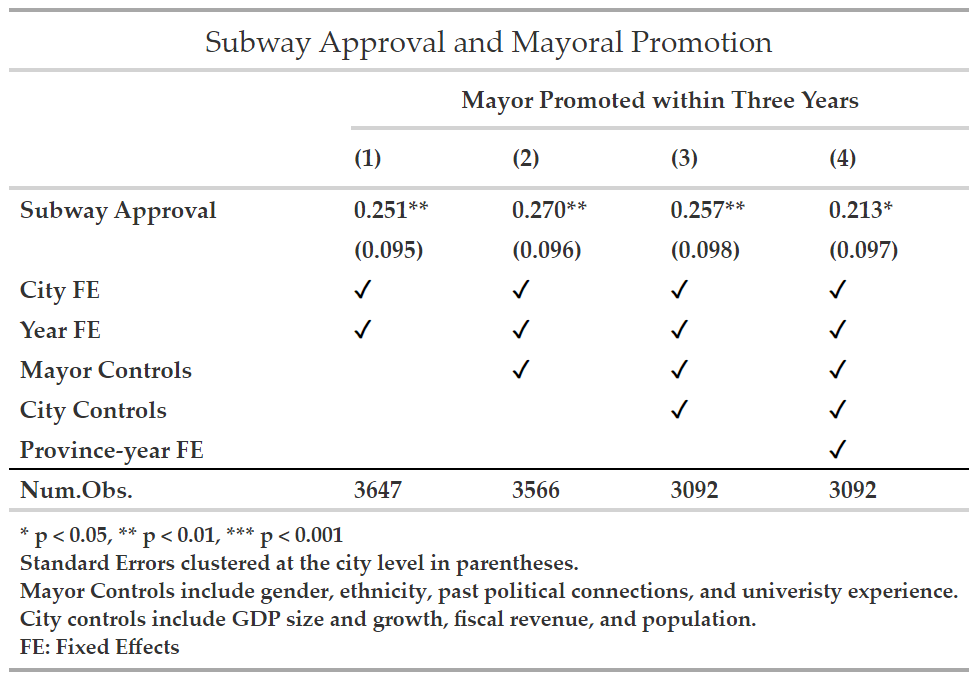
\includegraphics{tables/did_replication.png} \\
\end{longtable}

The results presented in Table~\ref{tbl-replication} illustrate the key
findings of the original difference-in-differences design by
\citet{lei2022private}. These results indicate a statistically
significant positive effect between a mayor securing approval for subway
infrastructure and their promotion within 3 years, across all
specifications of the design with increasing levels of controls.

On the base level, only including the fixed effects across city and
time, a mayor who has secured an approval for a subway construction will
see their chances of promotion in 3 years increase by 25 percentage
points, which is quite economically significant. The other
specifications also fall into this range of treatment effect, with the
lowest effect coming in when the model includes Province year fixed
effects.

Ensuring the validity of the difference-in-differences design requires
verifying the parallel trends assumption, which can be assessed through
the following model specification:
\[P_{ct} = \sum_{\substack{\gamma=-4 \\ \gamma \neq +1}}^{+5} \beta_{\gamma} Approval_{c(t+\gamma)} + \omega X_{ct-1} + \theta_c + \pi_t + \varepsilon_{it}\]
To establish a credible causal claim that obtaining a subway approval
heightens the chances of future promotion, it is imperative to confirm
that, in the absence of treatment, mayors who secured a subway approval
would have followed similar trends in their future promotion prospects
as those who did not receive the treatment.

\begin{figure}[tbp]

{\centering 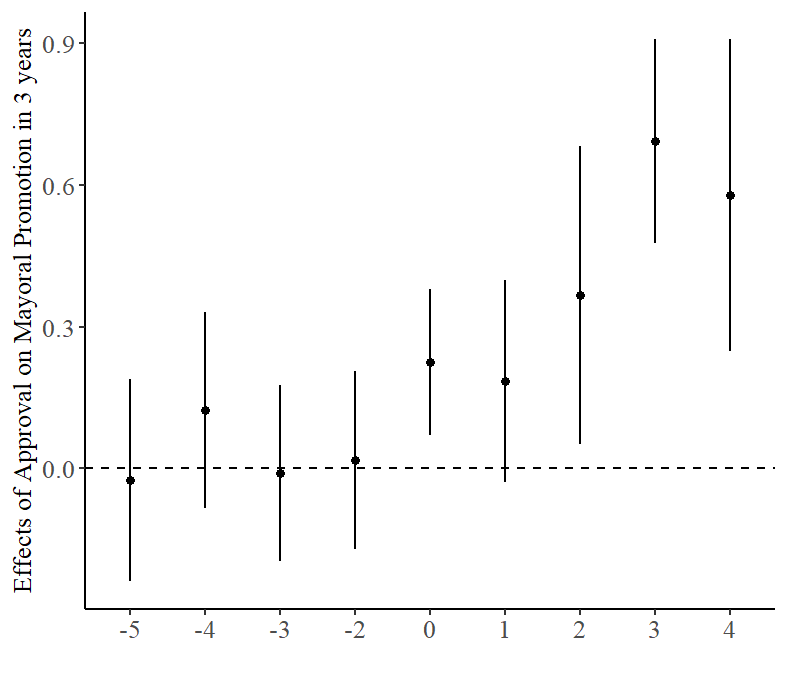
\includegraphics[width=0.7\textwidth,height=\textheight]{figures/parallel_trends.png}

}

\caption{\label{fig-parallel}Replication of \citet{lei2022private} Leads
and Lags Effect of Subway Approval on Future Promotion}

\end{figure}

Visualization of this concept through leads and lags, as depicted in
Figure~\ref{fig-parallel}, provides insights into the alignment of
trends among treated and untreated groups, substantiating the parallel
trends assumption. The leads serve as a placebo test to determine if
future treatment has any effect on present outcome, while lags
represents the effect of past treatment of present outcome. As evident
from Figure~\ref{fig-parallel}, wherein the year preceding the actual
treatment year serves as a baseline, the leads---extending up to five
years into the future---exhibit no statistically significant effect on
present outcomes. Notably, the estimate for the 4-year lead, although
showing an effect of approximately 0.15 (15 percentage points) on future
promotion, does not attain statistical significance.
Figure~\ref{fig-parallel} also shows us that securing a subway approval
in the past has a lasting effect on the promotion prospects of the city
mayors.

\hypertarget{heterogenous-effects-results-i-tenure}{%
\section{Heterogenous Effects Results I:
Tenure}\label{heterogenous-effects-results-i-tenure}}

I expand upon Lei \& Zhou's study by investigating heterogeneous
effects, beginning with an examination based on the mayor's tenure at
the time of securing approval for a subway infrastructure plan. This
analysis is encapsulated in the following ordinary least squares
regression:
\[P_{ct} = \alpha + \beta_{1}Approval + \beta_{2}Approval * Mayor Tenure + \gamma X_{c,t - 1} + \eta_{c} + \theta_{t} + \epsilon_{ct},\]

\hypertarget{tbl-extension2}{}
\begin{longtable}[]{@{}l@{}}
\caption{\label{tbl-extension2}Heterogeneous Effects Based on
Tenure}\tabularnewline
\toprule\noalign{}
\endfirsthead
\endhead
\bottomrule\noalign{}
\endlastfoot
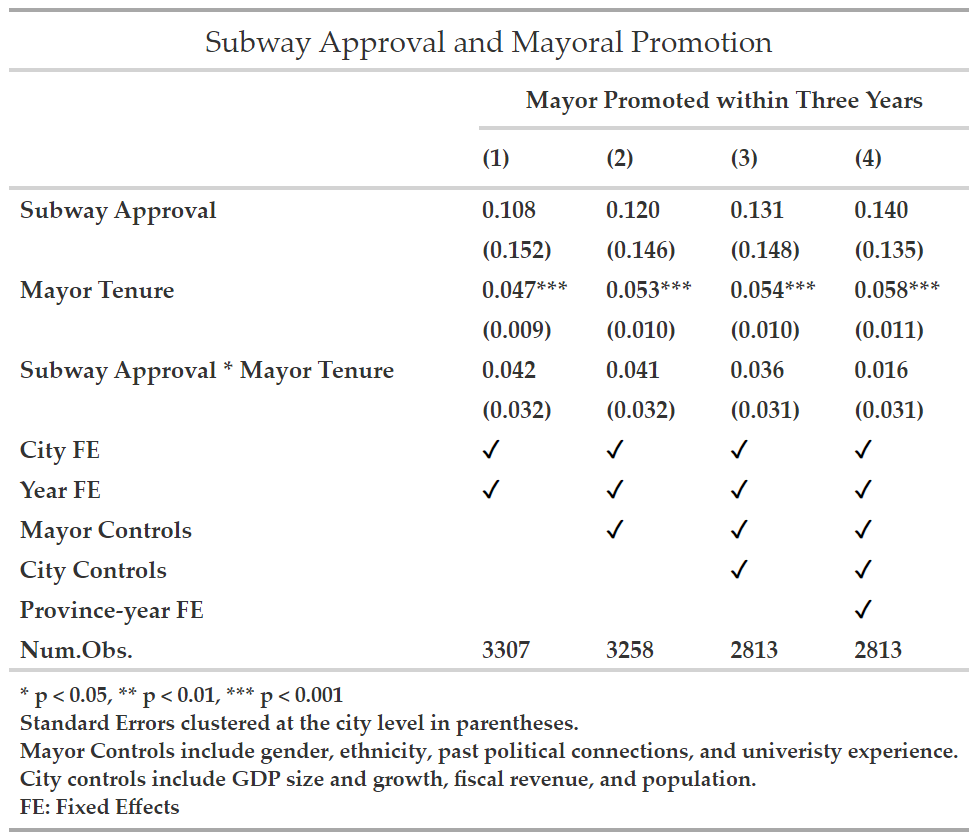
\includegraphics{tables/extension_tenure.png} \\
\end{longtable}

Table~\ref{tbl-extension2} shows the main results, from which we can see
that a mayor's tenure has a statistical significant effect on their
chances of future promotion through all specification of the difference
in difference model. This effect manifests as an increase ranging from
approximately 4.7 to 5.8 percentage points in the likelihood of future
promotion. It also shows us the effect of securing a subway approval
when a city mayor when a city mayor is in the initial stages of their
tenure (in other words, the coefficients on both the Mayor Tenure and
interaction term variables are zero). In these instances, the effects
are positive, spanning from 10.8 to 13.1 percentage points in increased
likelihood.

To discern the statistically significant effects of the specific
interaction between securing a subway approval and tenure,
Figure~\ref{fig-tenuremarg} illustrates the marginal effects of subway
approval based on tenure years, encompassing the first three models.
This visualization consistently portrays a positive effect of the
interaction between subway approval and tenure. Notably, mayors at the
outset of their careers, with minimal tenured experience, exhibit small
positive effects on future promotion when securing a subway approval,
though these effects are not statistically significant. As tenured years
increase, so does the impact of securing a subway approval on future
promotion. In fact, once a mayor surpasses 2.5 years in their position,
these positive effects become statistically significant, indicating an
increased likelihood of approximately 24 percentage points for future
promotion. This aligns with the earlier hypothesis suggesting that city
mayors stand a greater chance of promotion when they successfully secure
a subway approval during critical junctures in their careers,
specifically in their third and fourth tenure years. What's even more
intriguing is that the effect doubles to around a 50 percentage point
increase in probability after ten years of service. This contradicts the
previous notion that older politicians might face age discrimination, as
they could be considered too old for subsequent promotions.

\begin{figure}[tbp]

{\centering 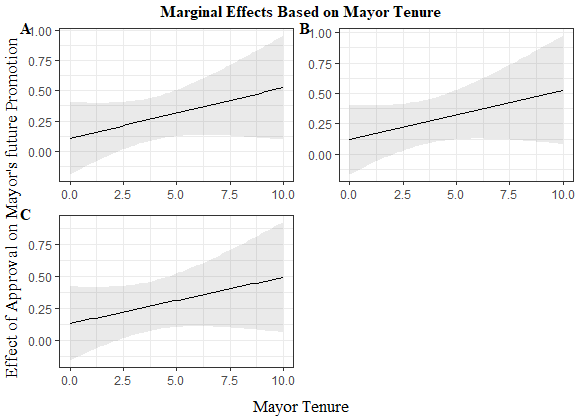
\includegraphics[width=0.7\textwidth,height=\textheight]{figures/marginaleffect_tenure.png}

}

\caption{\label{fig-tenuremarg}Marginal Effects Plot Based on
Interaction of Subway Approval with Mayor Tenure}

\end{figure}

The tenure distribution, illustrated in Figure~\ref{fig-tendist}, allows
for a visual identification of the most relevant effect for the majority
of the data. The graph indicates that a significant portion of the data
falls within the 0 to 4 years of tenure range, implying potential
effects of subway approval ranging from 0 to 27 percentage points.
Consequently, a substantial segment of the sample aligns closely with
the hypothesis that city mayors in their 3rd or 4th years have increased
chances of promotion when securing approval for a subway plan,
experiencing a noteworthy boost in their likelihood by 24 to 31
percentage points. In contrast, city mayors with less than 3 years in
office do not experience a notable increase in their promotion
prospects, even upon securing a subway approval. Interestingly, these
results highlight the fact that long-serving municipal mayors continue
to benefit from securing a subway approval, although such officials are
infrequent, as evident from the extended right tail observed in the
distribution plot. In summary, this study reveals significant
heterogeneous effects of subway approval on future promotion, contingent
on tenure, with the most pronounced impact observed for city mayors
during pivotal tenure years when they have the highest likelihood of
promotion.

\begin{figure}[tbp]

{\centering 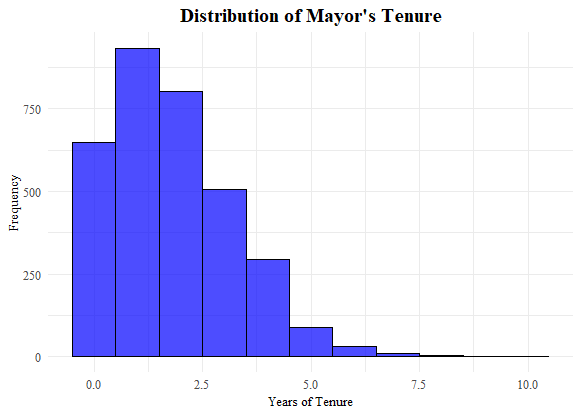
\includegraphics[width=0.7\textwidth,height=\textheight]{figures/tenure_dist.png}

}

\caption{\label{fig-tendist}Distribution of Mayor Tenure}

\end{figure}

\hypertarget{heterogenous-effects-results-ii-age}{%
\section{Heterogenous Effects Results II:
Age}\label{heterogenous-effects-results-ii-age}}

I explore a different form of heterogeneity based on the average age of
city mayors, as shown by the following regression using ordinary least
squares:
\[P_{ct} = \alpha + \beta_{1}Approval + \beta_{2}Approval * Age group + \gamma X_{c,t - 1} + \eta_{c} + \theta_{t} + \epsilon_{ct},\]

Table~\ref{tbl-extension} presents the primary outcomes of this
extension. Within the baseline group, securing a subway approval
markedly increased promotion chances by 27.5 percentage points,
demonstrating statistical significance and aligning with the findings of
the \citet{lei2022private} paper. The age groups of 30-35 and 35-40 were
excluded from the final model results due to a lack of observations
receiving the treatment, resulting in their interaction coefficients
being zero and subsequently dropped. While all other age groups,
excluding the 40-45 age group, exhibit lower chances in comparison, none
of these differences achieve statistical significance. Within the age
group 40-45, obtaining approval for subway construction in their city
yielded a detrimental impact on their likelihood of promotion in the
subsequent 3 years. To quantify, securing a subway approval decreased
their chances of promotion by 11.7 percentage points, and this effect
attains statistical significance across most specifications of the
design. However, it loses statistical significance when the model
incorporates province-year fixed effects, although the effect remains
negative.

\hypertarget{tbl-extension}{}
\begin{longtable}[]{@{}l@{}}
\caption{\label{tbl-extension}Heterogeneous Effects Based on
Age}\tabularnewline
\toprule\noalign{}
\endfirsthead
\endhead
\bottomrule\noalign{}
\endlastfoot
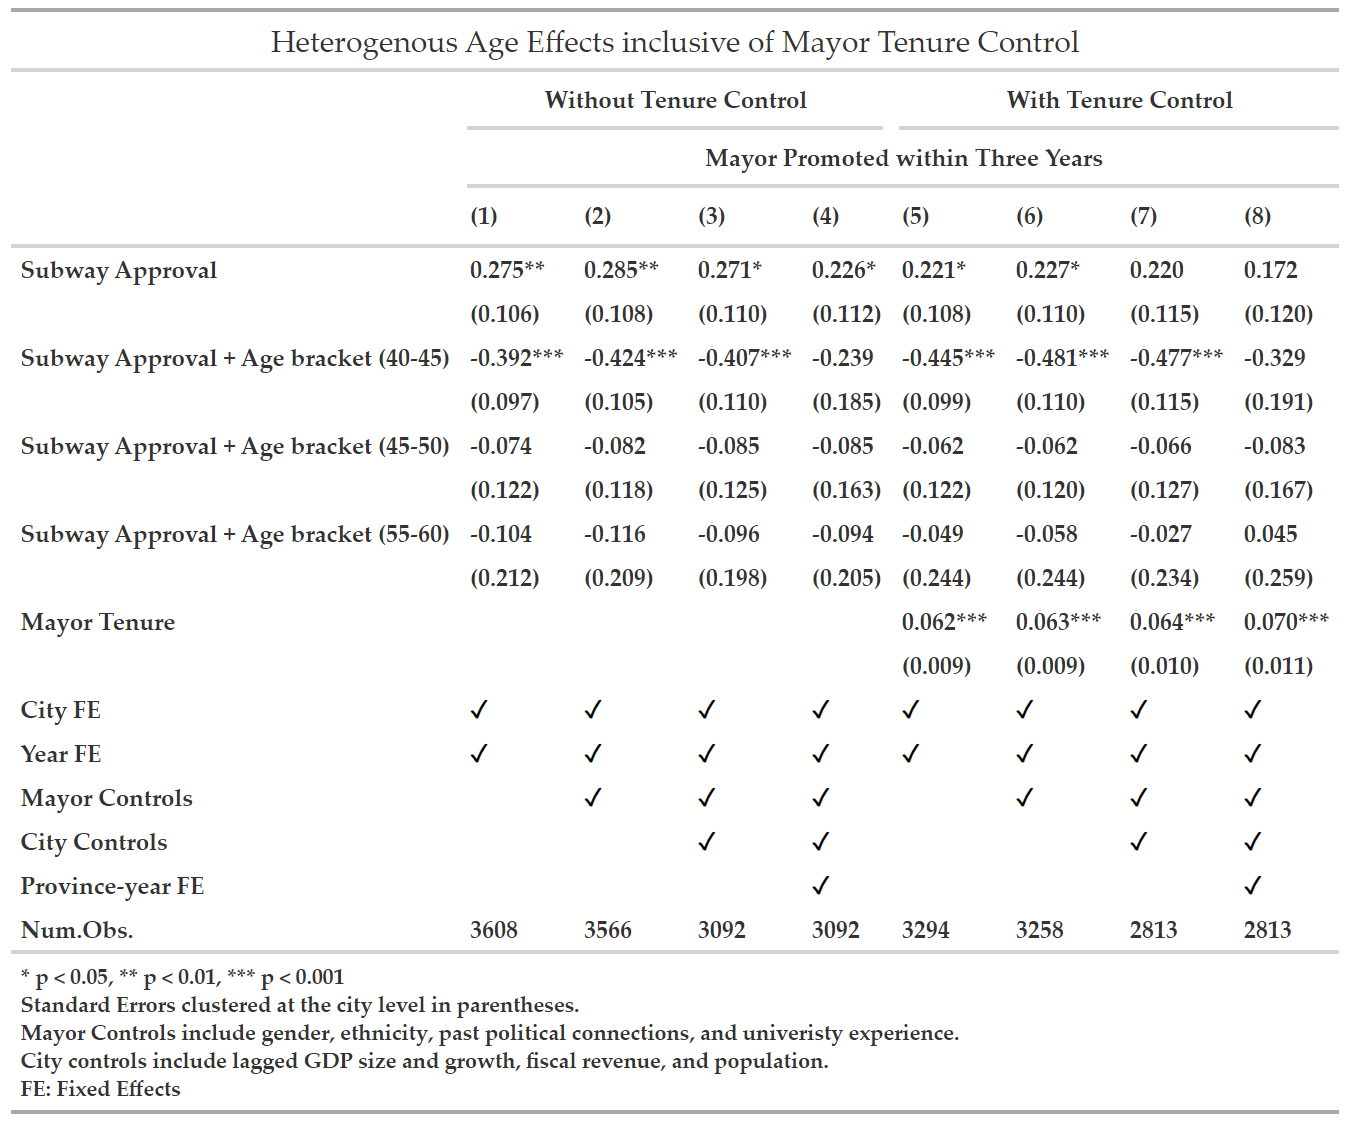
\includegraphics{tables/did_extension.png} \\
\end{longtable}

To ensure that the observed significant effects were not influenced by
outliers, I conducted a data filtration based on age groups. This
analysis aimed to assess the number of observations within each group
and determine how many actually received the treatment of securing a
subway approval. Upon investigation, I discovered that the statistical
differences observed in the 40-45 age group were primarily driven by a
single outlier, constituting only 1 observation out of a total of 410
observations within that group, representing approximately 0.2\% of the
total. In contrast, other age groups comprised 250 to 1480 observations,
with approximately 2-3\% receiving the treatment. Consequently, based on
this examination, I refrain from concluding that there is substantial
heterogeneity among the City Mayors included in this study based on age.

\hypertarget{conclusion}{%
\section{Conclusion}\label{conclusion}}

In conclusion, this study has successfully identified statistically
significant heterogeneous effects within the political exchange model in
Chinese local political systems, specifically focusing on the
influential factors of tenure and age. The results indicate a
significant variance in the effectiveness of securing subway approvals
based on tenure, with substantial implications for the promotion
prospects of city mayors in China. Notably, no statistically significant
differences were observed based on age, emphasizing the nuanced nature
of political dynamics.

Moving forward, there are promising avenues for further exploration.
Future research endeavors could extend this study by examining whether
similar heterogeneity exists for other infrastructure projects in China
or within different political exchange models in various countries.
Exploring these dimensions would not only contribute to a more
comprehensive understanding of political dynamics but also shed light on
the generalization of the findings beyond the scope of the current
study. Such investigations hold the potential to unveil broader patterns
and insights into the complex interplay between political exchanges,
tenure, and age in diverse political landscapes.

\newpage{}

\hypertarget{refs}{}

\begin{CSLReferences}{0}{0}\end{CSLReferences}


% END BODY %%%%%%%%%%%%%%%%%%%%%%%%%%%%%%%%%%%%%%%%%%%%%%%%%%%%%%%%%%%%%%%%%%%%%



\end{document}
